\documentclass{beamer}
\mode<presentation> {\usetheme{Madrid}}

\usepackage[utf8]{inputenc}
\usepackage{tikz}
\usepackage[export]{adjustbox}
\usepackage{amsmath}
\usepackage{appendixnumberbeamer}
\usepackage[absolute,overlay]{textpos}
\usepackage{subcaption}

\setbeamercolor{framesource}{fg=gray}
\setbeamerfont{framesource}{size=\tiny}
\setbeamertemplate{navigation symbols}{}
\setbeamercovered{transparent=00}
\setbeamerfont{footnote}{size=\tiny}

\newcommand{\todo}[1]{\textbf{\textcolor{red}{#1}}}
\newcommand{\me}[1]{\textcolor{gray}{#1}}
\newcommand{\source}[1]{\begin{textblock*}{4cm}(0.7cm,8.6cm)
	\begin{beamercolorbox}[ht=0.5cm,right]{framesource}
	\usebeamerfont{framesource}\usebeamercolor[fg]{framesource} Source: {#1}
	\end{beamercolorbox}
	\end{textblock*}
}

\title[short title]{Sol-gel ZrO$_2$ film optimized via Genetic Algorithm}
\author{Johann Dorn}
\begin{document}

%%%%% TITLEPAGE
\begin{frame}
 \titlepage
\end{frame}

\begin{frame}
	\frametitle[center]{Statistics}
		\begin{figure}
			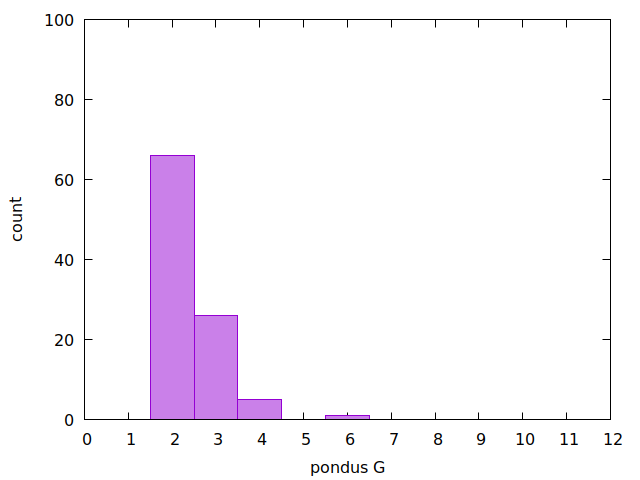
\includegraphics[width=.19\textwidth]{../../Data/I-V/I-V_131_2021_01_20/stat.png}
			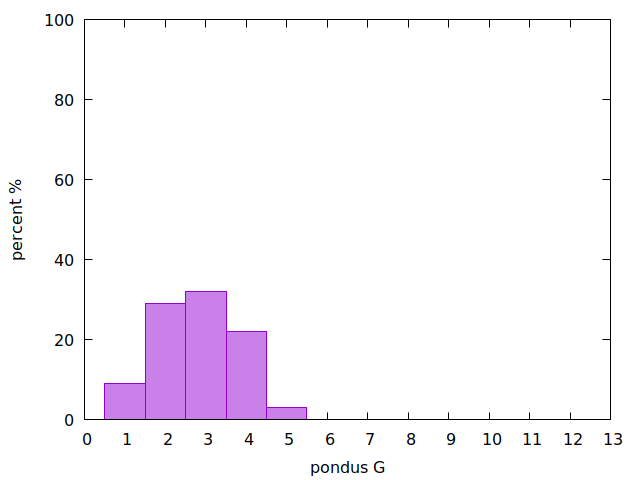
\includegraphics[width=.19\textwidth]{../../Data/I-V/I-V_135_2021_01_20/stat.png}
			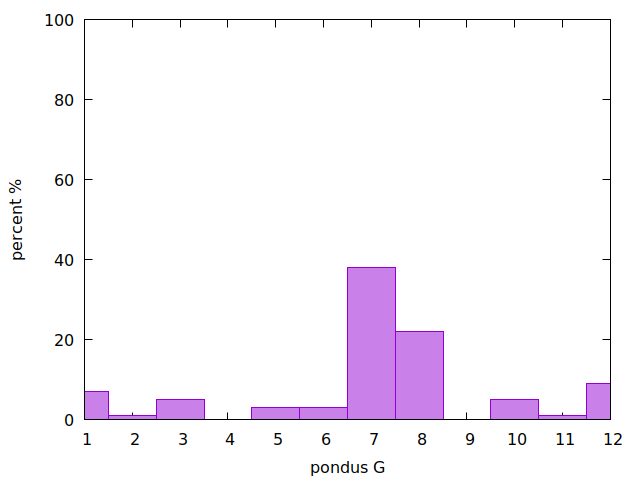
\includegraphics[width=.19\textwidth]{../../Data/I-V/I-V_146_2021-02-23/stat.png}
%			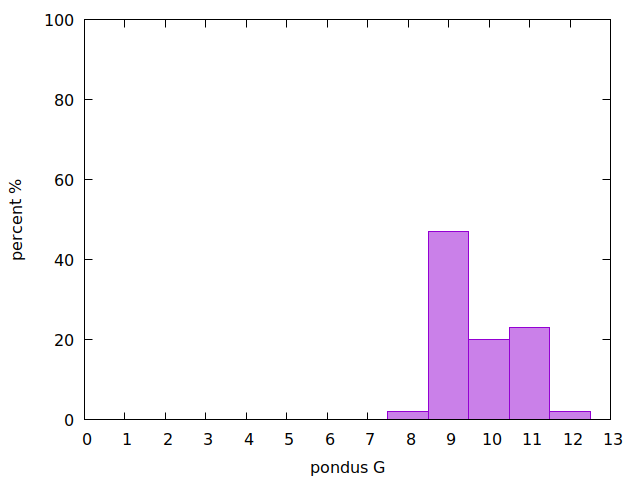
\includegraphics[width=.19\textwidth]{../../Data/I-V/I-V_150_2021_02_03/stat.png}
			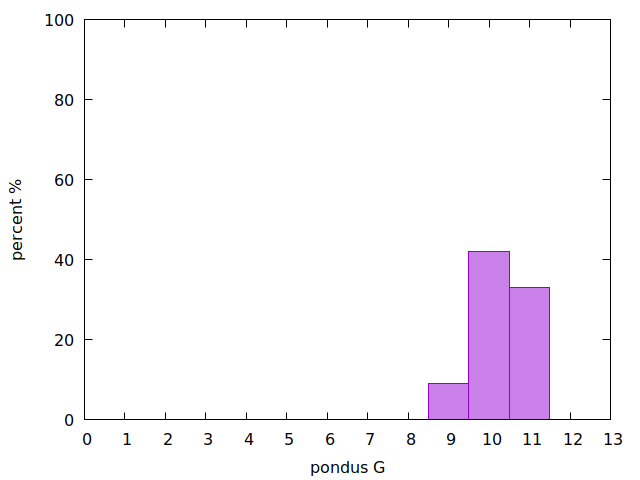
\includegraphics[width=.19\textwidth]{../../Data/I-V/I-V_150_2021_02_09/stat.png}
			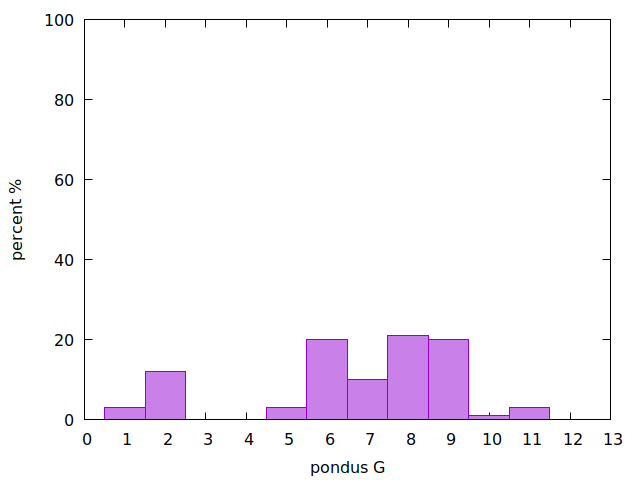
\includegraphics[width=.19\textwidth]{../../Data/I-V/I-V_151_2021_02_05/stat.png}
			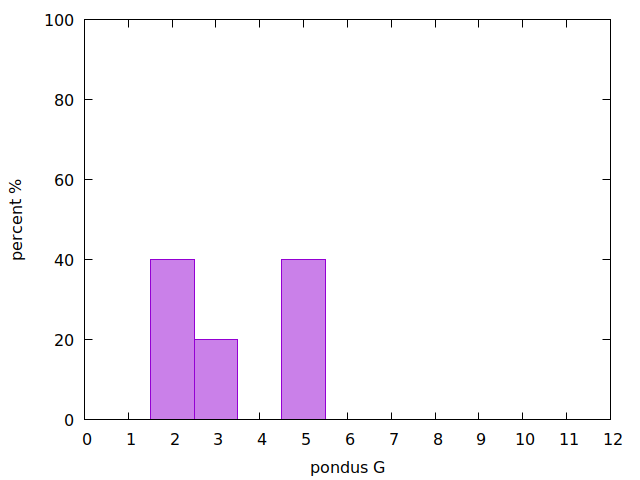
\includegraphics[width=.19\textwidth]{../../Data/I-V/I-V_152_2021_02_09/stat.png}
			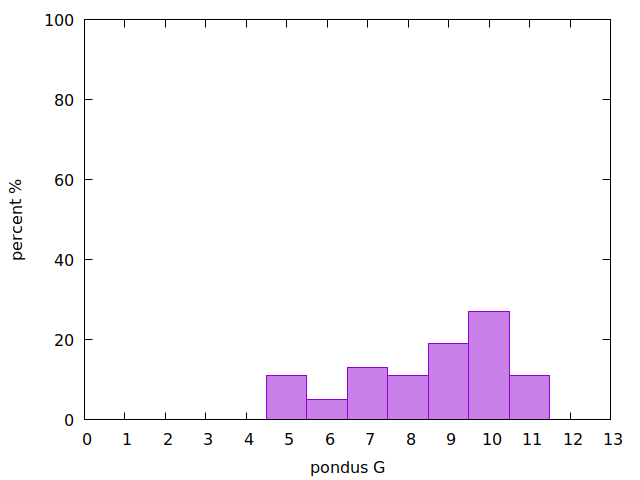
\includegraphics[width=.19\textwidth]{../../Data/I-V/I-V_153_2021_03_03/stat.png}
			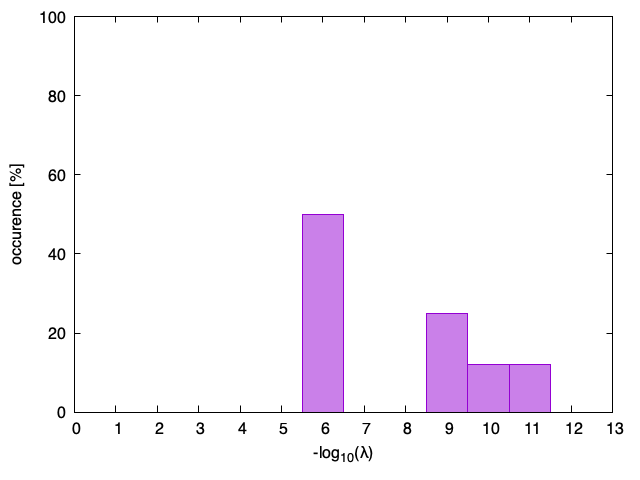
\includegraphics[width=.19\textwidth]{../../Data/I-V/I-V_154_2021_02_23/stat.png}
			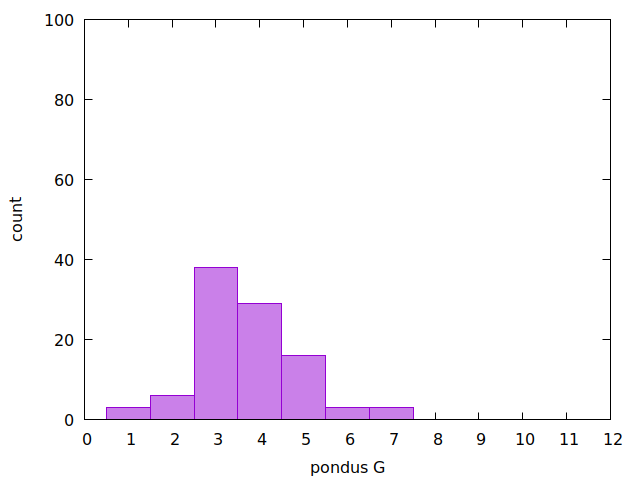
\includegraphics[width=.19\textwidth]{../../Data/I-V/I-V_156_2021_02_23/stat.png}
			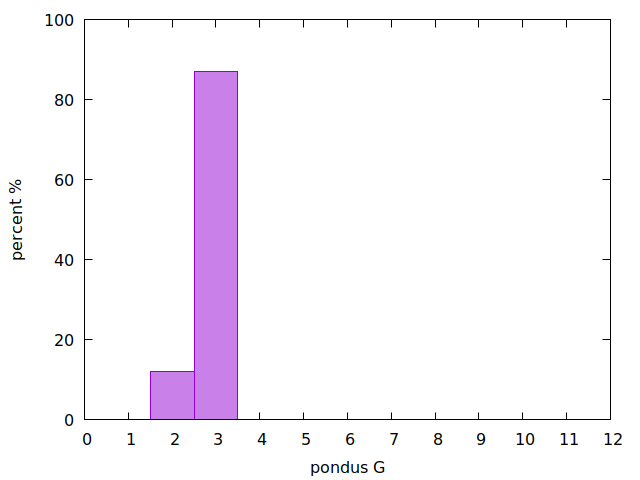
\includegraphics[width=.19\textwidth]{../../Data/I-V/I-V_157_2021_02_25/stat.png}
			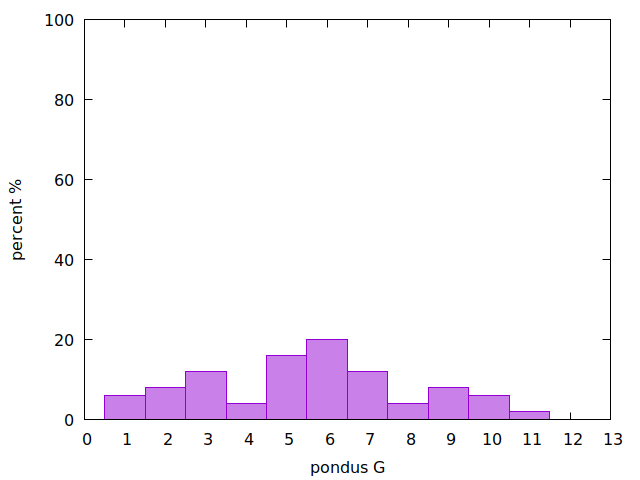
\includegraphics[width=.19\textwidth]{../../Data/I-V/I-V_158_2021_02_26/stat.png}
			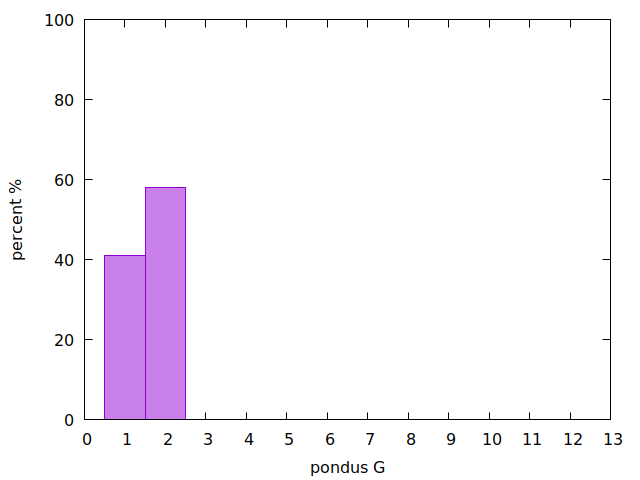
\includegraphics[width=.19\textwidth]{../../Data/I-V/I-V_160_2021_03_01/stat.png}
			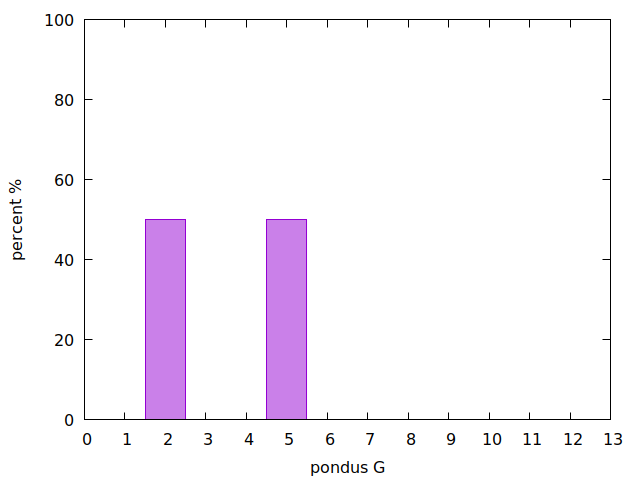
\includegraphics[width=.19\textwidth]{../../Data/I-V/I-V_161_milky_2021_03_01/stat.png}
			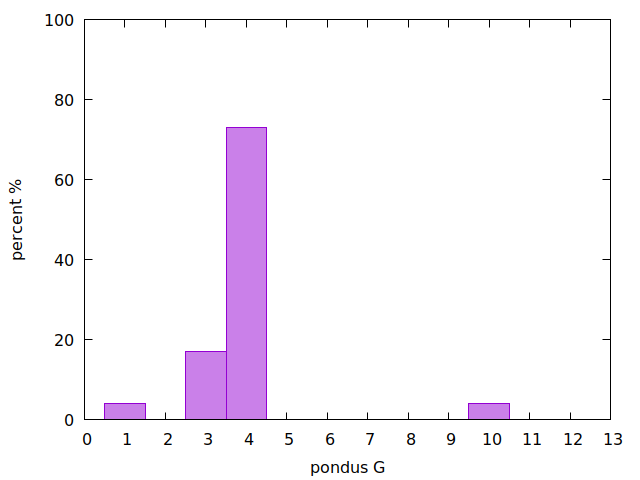
\includegraphics[width=.19\textwidth]{../../Data/I-V/I-V_186_2021_03_01/stat.png}
			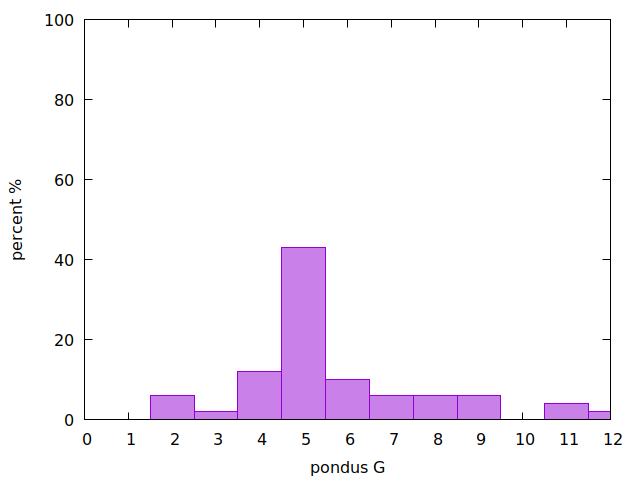
\includegraphics[width=.19\textwidth]{../../Data/I-V/I-V_187_2021_03_03/stat.png}
			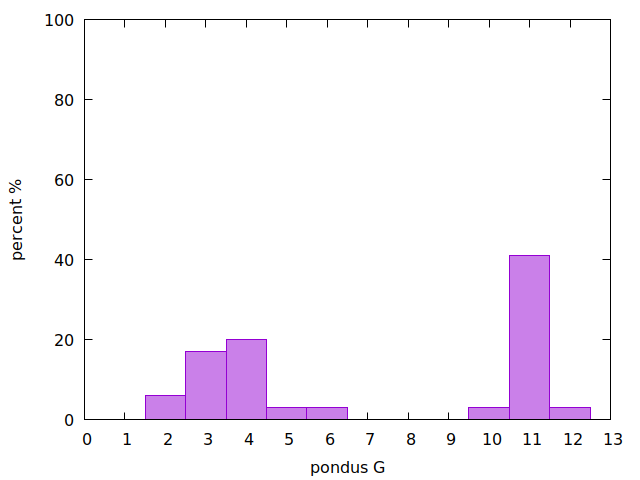
\includegraphics[width=.19\textwidth]{../../Data/I-V/I-V_188_2021_03_03/stat.png}
			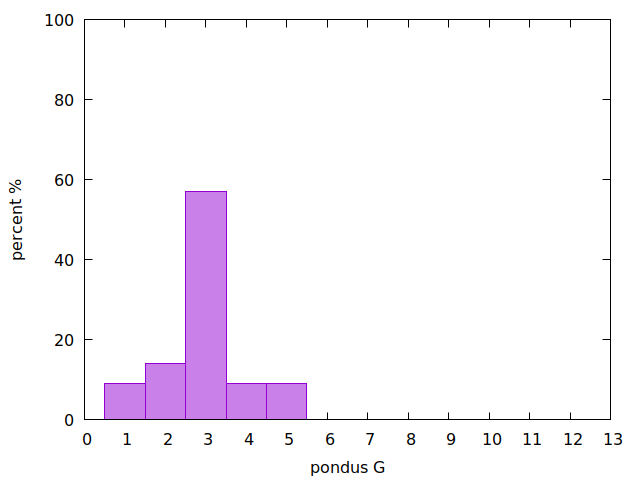
\includegraphics[width=.19\textwidth]{../../Data/I-V/I-V_190_2021_03_04/stat.png}
			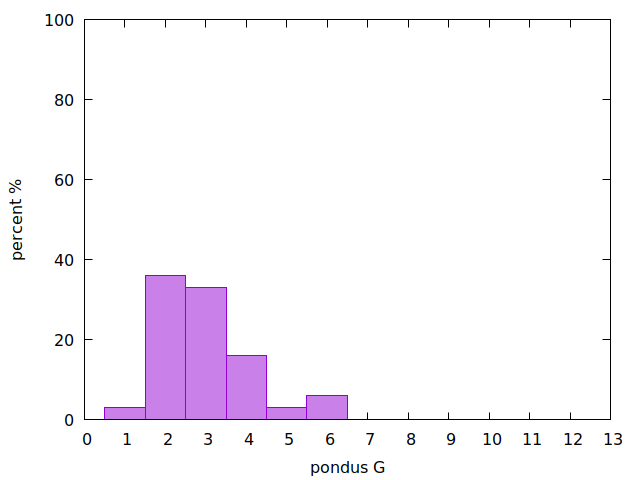
\includegraphics[width=.19\textwidth]{../../Data/I-V/I-V_194_2021_03_04/stat.png}
			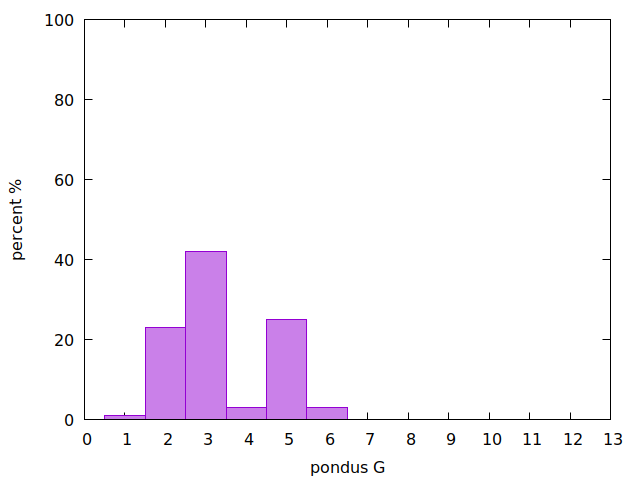
\includegraphics[width=.19\textwidth]{../../Data/I-V/I-V_195_2021_03_04/stat.png}
			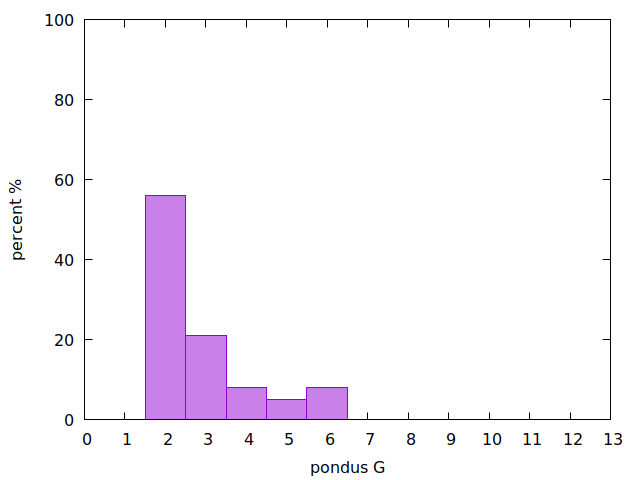
\includegraphics[width=.19\textwidth]{../../Data/I-V/I-V_198_2021_03_04/stat.png}
		\end{figure}
\end{frame}

\begin{frame}
	\frametitle[center]{Calculation}
	\begin{columns}[t]
		\column{0.49\textwidth}
		\begin{figure}
			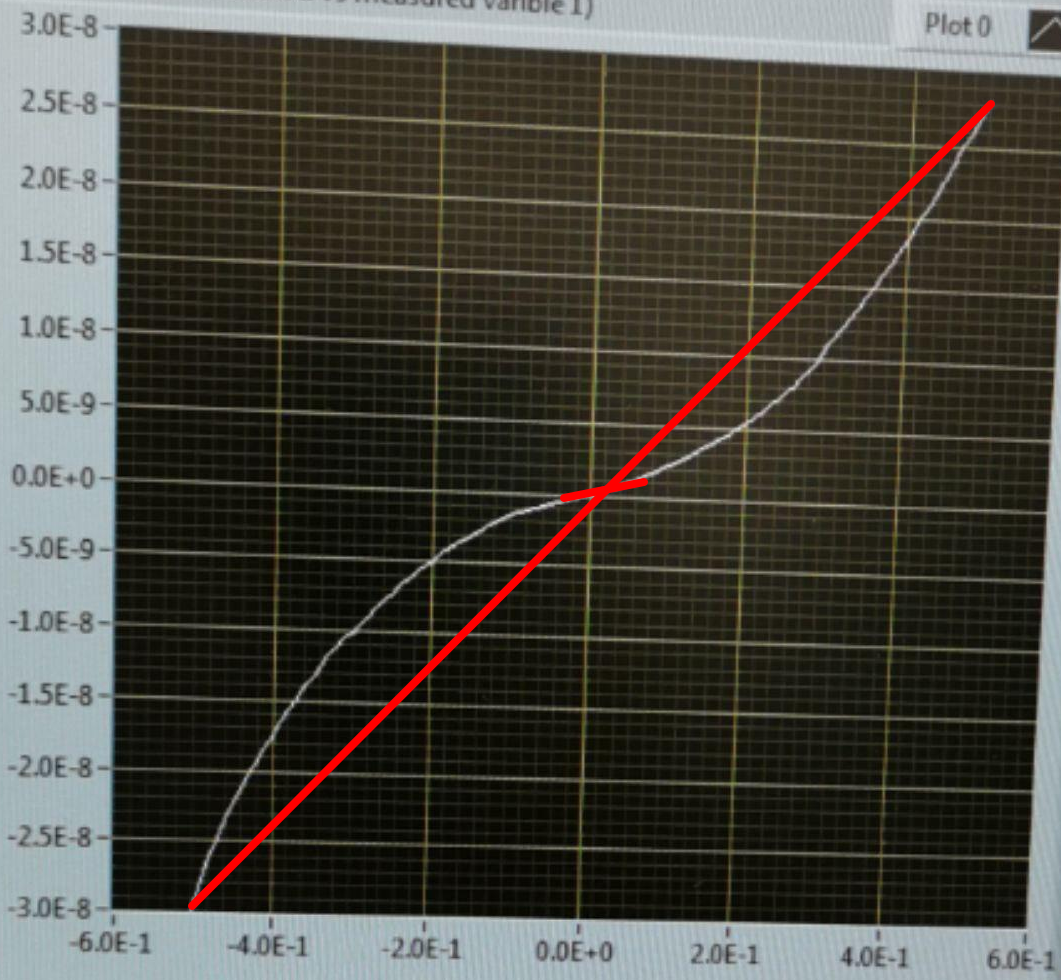
\includegraphics[width=.9\textwidth]{pics/iv_grad.png}
		\end{figure}
	\column{0.49\textwidth}
	\begin{itemize}
		\item G = $\frac{dI}{dV}$ = 4.234E-6
		\item G' = log($|$G$|$) = -5.37
		\item pG = -log($|$G$|$) = 5.37 \me{pondus,power,potential}
%		\item pG = 5.37 \me{$\rightarrow$ 5}
		\item Q: which points best for dV
		\item min max overestimation ? 
		\item average ?
	\end{itemize}
	\end{columns}
\end{frame}

\begin{frame}
	\frametitle[center]{Best of}
		\begin{figure}
			\begin{subfigure}{.32\textwidth}
				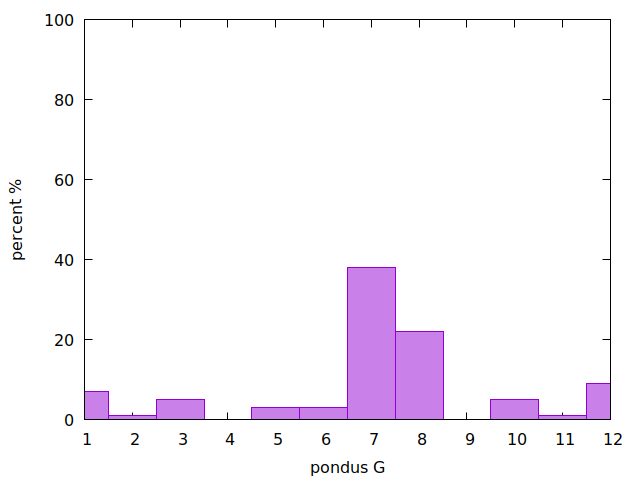
\includegraphics[width=.99\textwidth]{../../Data/I-V/I-V_146_2021-02-23/stat.png}
				\caption{146, 10x1F HG}
			\end{subfigure}
			\begin{subfigure}{.32\textwidth}
				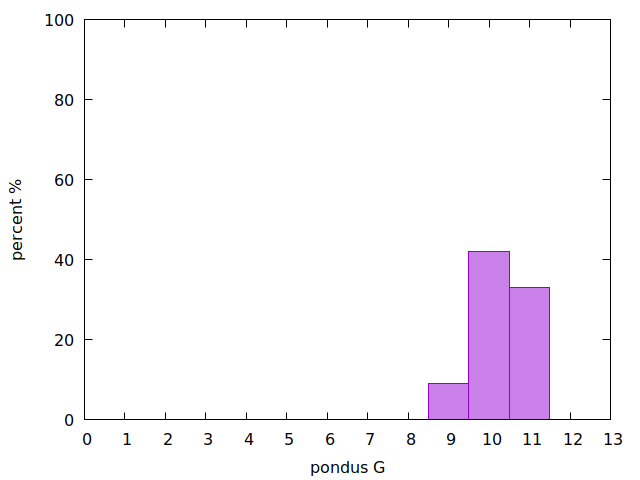
\includegraphics[width=.99\textwidth]{../../Data/I-V/I-V_150_2021_02_09/stat.png}
				\caption{150, 5x2F HG}
			\end{subfigure}
			\begin{subfigure}{.32\textwidth}
				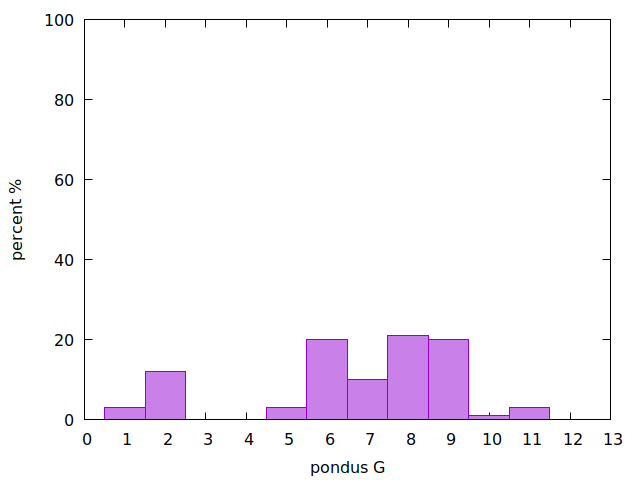
\includegraphics[width=.99\textwidth]{../../Data/I-V/I-V_151_2021_02_05/stat.png}
				\caption{151, 2x2F HG}
			\end{subfigure}
			\begin{subfigure}{.32\textwidth}
				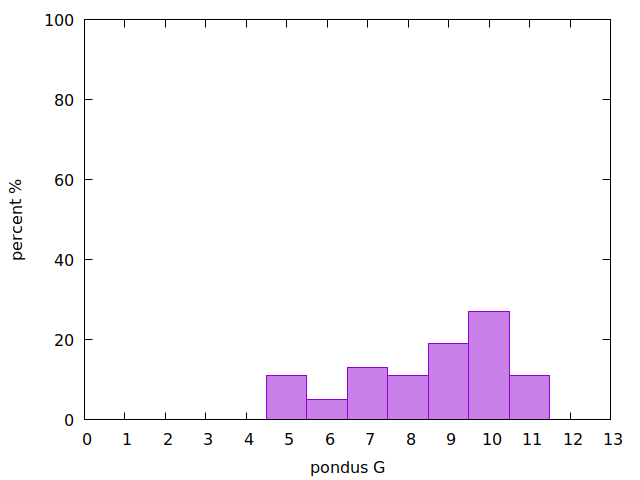
\includegraphics[width=.99\textwidth]{../../Data/I-V/I-V_153_2021_03_03/stat.png}
				\caption{153, 3x4F HG}
			\end{subfigure}
			\begin{subfigure}{.32\textwidth}
				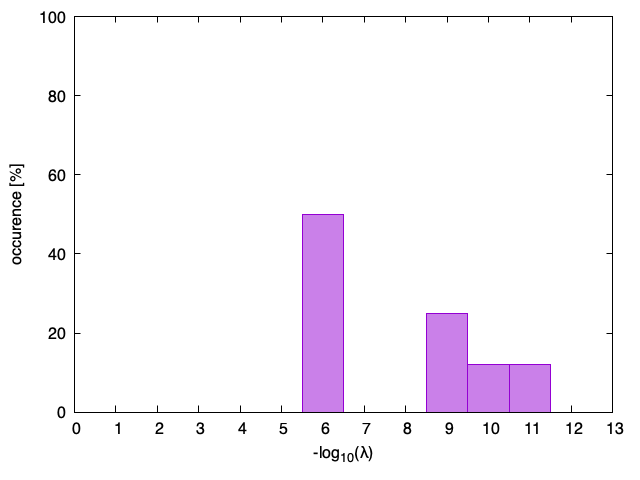
\includegraphics[width=.99\textwidth]{../../Data/I-V/I-V_154_2021_02_23/stat.png}
				\caption{154, 3x4F HG}
			\end{subfigure}
			\begin{subfigure}{.32\textwidth}
				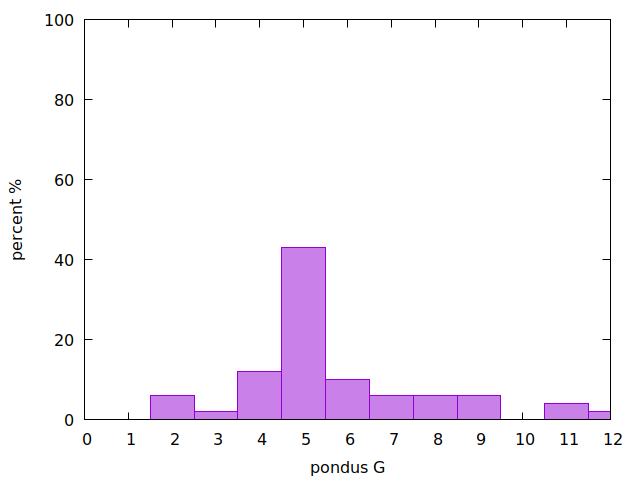
\includegraphics[width=.99\textwidth]{../../Data/I-V/I-V_187_2021_03_03/stat.png}
				\caption{187, 10x1F 5mm/s }
			\end{subfigure}
		\end{figure}
\end{frame}

\begin{frame}
	\frametitle{All questions}
	\begin{itemize}
		\item where should be threshold be for holes?
		\item how to calculate derivative?
		\item boundaries for Tcal = [300:500] \me{[400:500]} $^o$C
		\item layers  = [6:14] \me{[4:10]} 
		\item conc = [2:5] \me{[1:5]}
		\item vDoc = [10:20] mm/s
		\item TDOC = [40:80] $^o$C
		\item vCal = [2:16] $^o$C/min
		\item 
	\end{itemize}
\end{frame}

	

%%%%%%%%%%%%%%%%%%%%%%%%%%%%%%%%%%%%%%%%%%%%%%%%%%%%%%%%%%%%%%%%%%%%%
\iffalse
\begin{frame}
 \frametitle{Overview \todo{just for me}}
	\begin{itemize}
		\item What is the goal
		\item What is the status
		\item What are the optimazable parameters
		\item What is a genetic algorithm 
		\item What are the parameters for a GA
		\item Plan 
	\end{itemize}
\end{frame}

\begin{frame}
	\frametitle{What is the goal?}
	\begin{itemize}
		\item ZrO$_2$ film via doctor blading on steel 
		\item should be insulating (no cracks or holes)
		\item minimum thickness of 200 $\mu$m
	\end{itemize}
\end{frame}

\begin{frame}
	\frametitle{What is the status?}
	\begin{itemize}
		\item lower heating rate produces less cracks
		\item composition of starting solution
	\end{itemize}
\end{frame}

\begin{frame}
	\frametitle{What are optimizable parameters?}
	\begin{columns}[t]
		\column{0.49\textwidth}
			\begin{itemize}
				\item Volume:
				\begin{itemize}
					\item Zr isopropoxide 
					\item AcAc
					\item iPrOH
					\item H2O
					\item \me{Base? organic? for pH regulation}
					\item \me{Acid?}
					\item \me{Surfactant?}
					\item \me{high molecular co-polymer?}
				\end{itemize}
			\end{itemize}
			\pause
		\column{0.49\textwidth}
			\begin{itemize}
				\item Time:
				\begin{itemize}
					\item Mixing Time
					\item \me{waiting before spreading}
				\end{itemize}
				\item Temperature:
				\begin{itemize}
					\item Heating rate
					\item Calcination holding time
					\item \me{Max temperature}
					\item \me{Heating method oven/hot plate}
				\end{itemize}
			\end{itemize}
	\end{columns}
\end{frame}

\begin{frame}
	\frametitle{What is a genetic algorithm?}
	\begin{itemize}
		\item population of individuals (experiments)
		\item genes (experiment parameters)
		\item fitness (grade of satisfying the demands)
		\item only the fittest survive
		\item the individuals pair and produce offspring
		\item mutations
	\end{itemize}
\end{frame}

\begin{frame}
	\frametitle{How does a GA work?}
	\begin{enumerate}
		\item random initial population
		\item calculate fitness
		\item select pairs to become parents
		\item mixing of their genomes via cross over
		\item mutate the offspring genomes
		\item replace old with new population
		\item go to step 2
	\end{enumerate}
\end{frame}

\begin{frame}
	\frametitle{What are the parameters for GA?}
	\begin{itemize}
		\item size of initial population (2-4 fold of genes)
		\item how is the fitness calculated?
		\item how are the parent pairs selected?
		\item crossover probability or rate
		\item mutation rate
		\item how is the population replaced?
	\end{itemize}
\end{frame}

\begin{frame}
	\frametitle{Plan}
	\begin{itemize}
		\item 6 month \~=  24 weeks
%		\item 2 weeks experimentally explore search space (+ writing of code)
		\item First 2 weeks:
			\begin{itemize}
				\item experimentally explore search space
				\item choose parameters
				\item choose GA parameters and write code
			\end{itemize}
		\item 20 weeks: 10-20 generations\\
			create data for generations
		\item 2 weeks buffer
	\end{itemize}
\end{frame}

%%%%%%%%%%%%%%%%%%%%%%%%%%%%%%%%%%%%%%%%%%%%%%%%%%%%%%%%%%%%%%%%%%%%%
\begin{frame}
	\frametitle[center]{Introduction}
	\textbf{Confinement Effect of Sub-nanometer Difference on Melting Point of Ice-Nanotubes Measured by Photoluminescence Spectroscopy} - Shohei Chiashi et al. (ACS Nano 2019, 13, 1177-1182)
	\begin{columns}[t]
		\column{0.49\textwidth}
		\begin{itemize}
			\item some thing
		\end{itemize}

		\column{0.49\textwidth}
		\begin{figure}
			\includegraphics[width=.5\textwidth]{tiger}
			\source{ACS Nano 2019, 13, 1177-1182}
		\end{figure}
	\end{columns}
\end{frame}

\begin{frame}
	\frametitle[center]{Single Walled Carbon Nano Tubes (SWCNT)}
	\begin{columns}[t]
		\column{0.49\textwidth}
		\begin{figure}
			\includegraphics<1>[width=.9\textwidth]{example-image-a}
			\includegraphics<2->[width=.9\textwidth]{example-image-b}
			\source{source}
		\end{figure}
	\column{0.49\textwidth}
		\begin{figure}
			\includegraphics<3->[width=.9\textwidth, right]{example-image-c}
		\end{figure}
		\pause
		\visible<4>{(3,1) SWCNT}
	\end{columns}
\end{frame}

%%%%%%%%%%%%%%%%%%%%%%%%%%%%%%%%%%%%%%%%%%%%%%%%%%%%%%%%%%60

\appendix
\begin{frame}
	\frametitle{Frequency Dependence of Permitivity}
\end{frame}
\fi

\end{document}
